

\begin{figure}[t] 
	\centering
	\begin{minipage}[b]{0.47\textwidth}
    	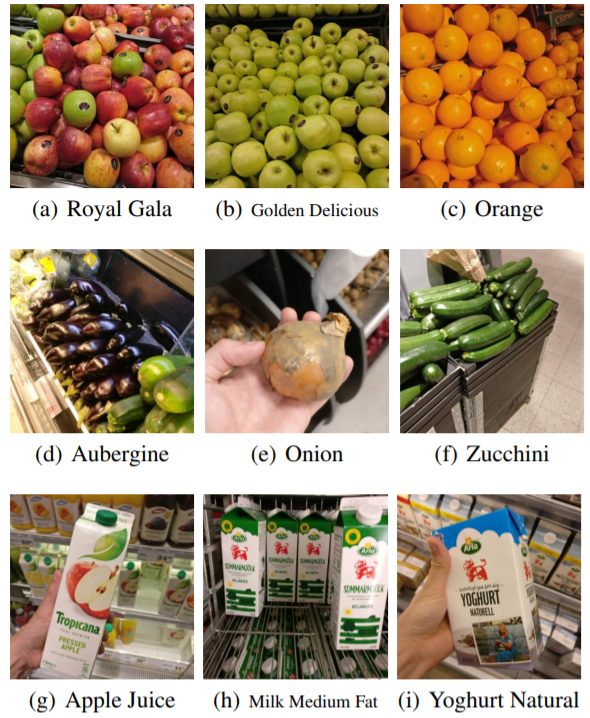
\includegraphics[scale=0.5]{PaperB/figures_and_tables/figure1.png}
		\caption{Examples of natural images in our dataset, where each image has been taken inside a grocery store. Image examples of fruits, vegetables, and refrigerated products are presented in each row respectively.}
		\label{fig:dataset_figures}
	\end{minipage}
	\hspace{10pt}
	%\vspace{-10mm}
	\begin{minipage}[b]{0.47\textwidth}
		\centering
	    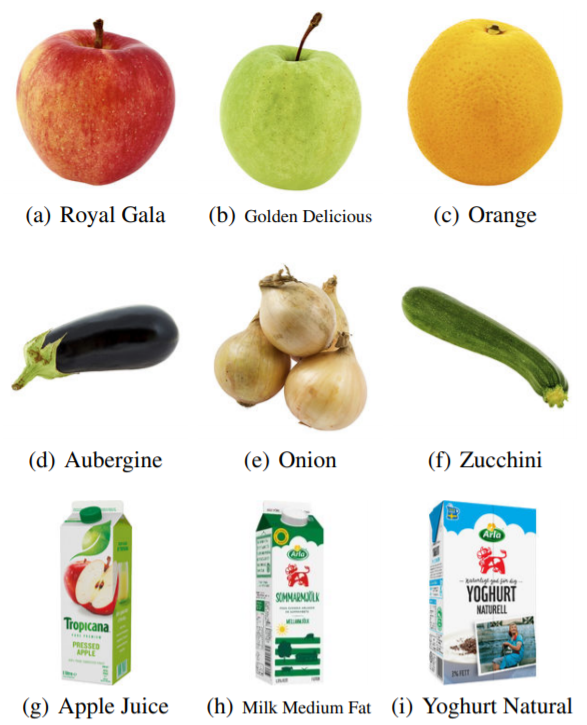
\includegraphics[scale=0.5]{PaperB/figures_and_tables/figure2.png}
		\caption{Examples of iconic images downloaded from a grocery shopping website, which corresponds to the target items in the images in Figure \ref{fig:dataset_figures}. \newline}
		\label{fig:iconic_image_figures}
	\end{minipage} 
	\vspace{-2mm}
\end{figure}



\begin{comment}

\begin{figure}
    \centering
    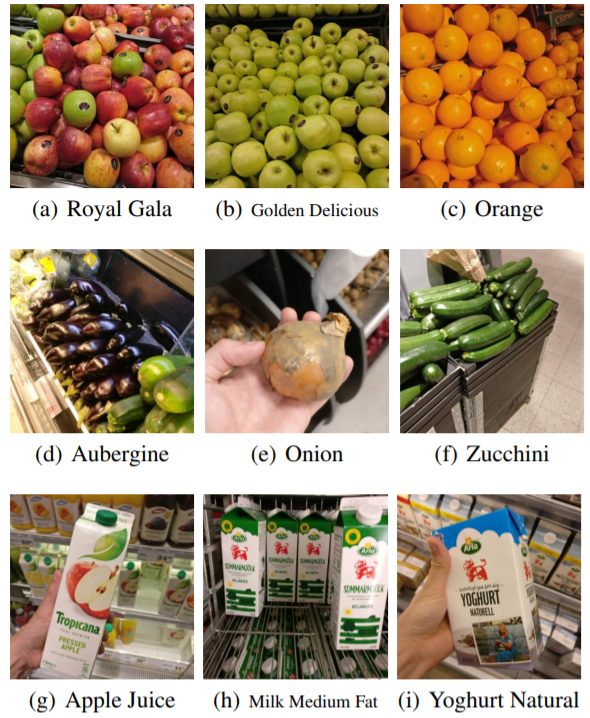
\includegraphics[scale=0.5]{PaperB/figures_and_tables/figure1.png}
    \caption{Examples of natural images in our dataset, where each image has been taken inside a grocery store. Image examples of fruits, vegetables, and refrigerated products are presented in each row respectively.}
    \label{fig:dataset_figures}
\end{figure}

\begin{figure}
    \centering
    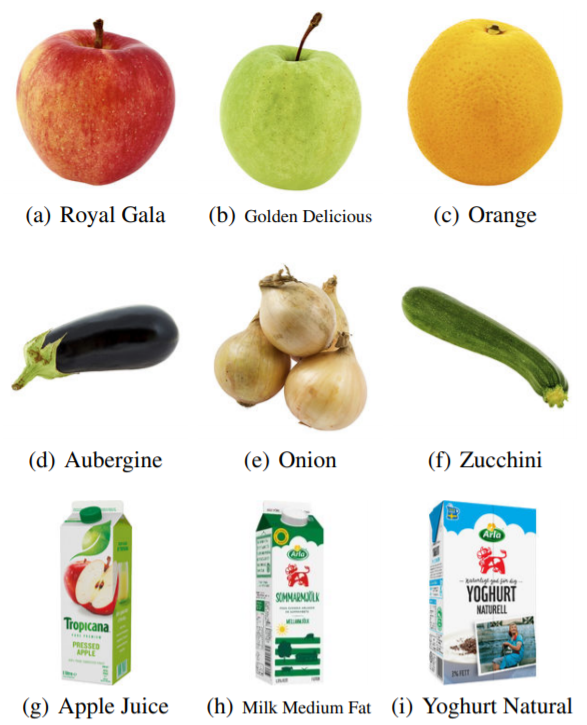
\includegraphics[scale=0.5]{PaperB/figures_and_tables/figure2.png}
    \caption{Examples of iconic images downloaded from a grocery shopping website, which corresponds to the target items in the images in Figure \ref{fig:dataset_figures}.}
    \label{fig:iconic_image_figures}
\end{figure}.
\end{comment}

